% vim: set tw=78 tabstop=4 shiftwidth=4 aw ai:
\documentclass{beamer}

\usepackage[utf8x]{inputenc}		% diacritice
\usepackage[english]{babel}
\usepackage{color}			% highlight
\usepackage{alltt}			% highlight

\usepackage{hyperref}			% folosiți \url{http://...}
					% sau \href{http://...}{Nume Link}
\usepackage{verbatim}

\mode<presentation>
{ \usetheme{Berlin} }

% Încărcăm simbolurilor Unicode românești în titlu și primele pagini
\PreloadUnicodePage{200}

% Arătăm numărul frame-ului
\newcommand{\frameofframes}{/}
\newcommand{\setframeofframes}[1]{\renewcommand{\frameofframes}{#1}}

\setframeofframes{of}
\makeatletter
\setbeamertemplate{footline}
  {%
    \begin{beamercolorbox}[colsep=1.5pt]{upper separation line foot}
    \end{beamercolorbox}
    \begin{beamercolorbox}[ht=2.5ex,dp=1.125ex,%
      leftskip=.3cm,rightskip=.3cm plus1fil]{author in head/foot}%
      \leavevmode{\usebeamerfont{author in head/foot}\insertshortauthor}%
      \hfill%
      {\usebeamerfont{institute in head/foot}\usebeamercolor[fg]{institute in head/foot}\insertshortinstitute}%
    \end{beamercolorbox}%
    \begin{beamercolorbox}[ht=2.5ex,dp=1.125ex,%
      leftskip=.3cm,rightskip=.3cm plus1fil]{title in head/foot}%
      {\usebeamerfont{title in head/foot}\insertshorttitle}%
      \hfill%
      {\usebeamerfont{frame number}\usebeamercolor[fg]{frame number}\insertframenumber~\frameofframes~\inserttotalframenumber}
    \end{beamercolorbox}%
    \begin{beamercolorbox}[colsep=1.5pt]{lower separation line foot}
    \end{beamercolorbox}
  }
\makeatother

\setbeamertemplate{navigation symbols}{}%remove navigation symbols

\title[Comparative Analysis of Congestion Algorithm
Influence on OpenVPN-MPTCP Performance]{Comparative Analysis of Congestion
Algorithm Influence on OpenVPN-MPTCP Performance}
\subtitle{Master Report Session -- February 2015}
\institute{Faculty of Automatic Control and Computers,\\
	University POLITEHNICA of Bucharest}
\author[Silviu Petria, Silviu-Mihai Popescu]{Silviu Petria, Silviu-Mihai
Popescu\\
	Supervisor: Costin Raiciu}
\date{February 7, 2015}

\begin{document}

% Slide-urile cu mai multe părți sunt marcate cu textul (cont.)
\setbeamertemplate{frametitle continuation}[from second]

\frame{\titlepage}

\section{Congestion Control Algorithms}
\begin{frame}{Congestion Control Algorithms}
  \begin{itemize}
    \item OLIA
    \begin{itemize}
      \item coarse-grained
      \item packet loss
    \end{itemize}
    \item wVegas
    \begin{itemize}
      \item fine-grained
      \item packet delay
    \end{itemize}
  \end{itemize}
\end{frame}

\section{Revised Testbed}
\begin{frame}{Revised Testbed}
  \begin{figure}
    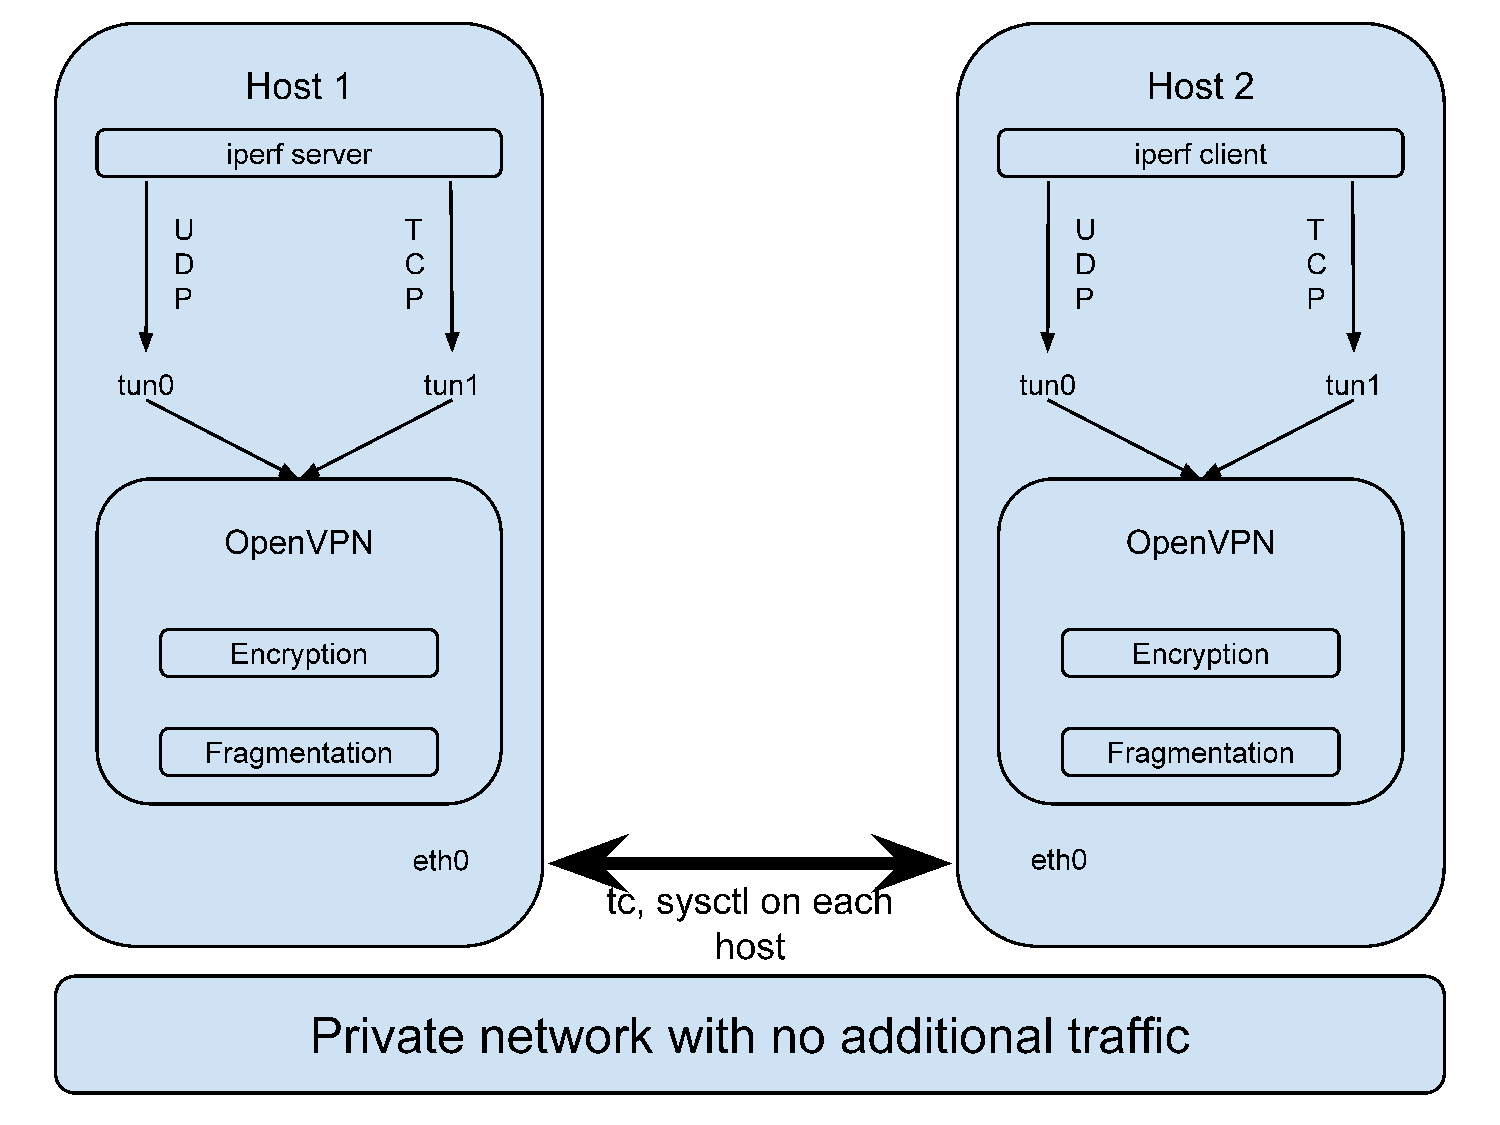
\includegraphics[scale=0.35]{img/mptcp-openvpn-bare}
  \end{figure}
\end{frame}

\section{OLIA Behavior}
\begin{frame}{OLIA Behavior - Single TCP Tunnel}
  \begin{figure}
    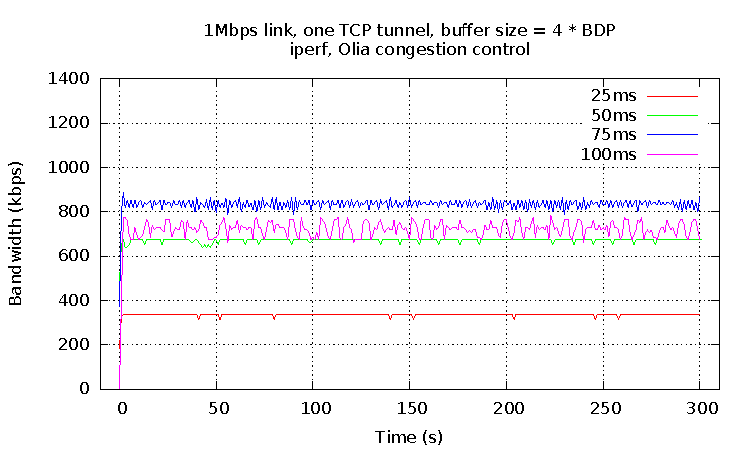
\includegraphics[scale=0.75]{img/olia-tcp-4}
  \end{figure}
\end{frame}
\begin{frame}{OLIA Behavior - Two Tunnels}
  \begin{figure}
    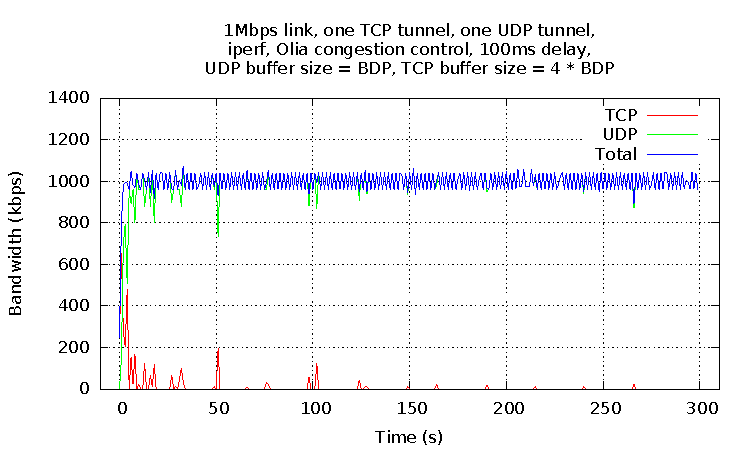
\includegraphics[scale=0.75]{img/olia-mptcp-100ms-4}
  \end{figure}
\end{frame}
\begin{frame}{OLIA Behavior - WiFi/3G}
  \begin{figure}
    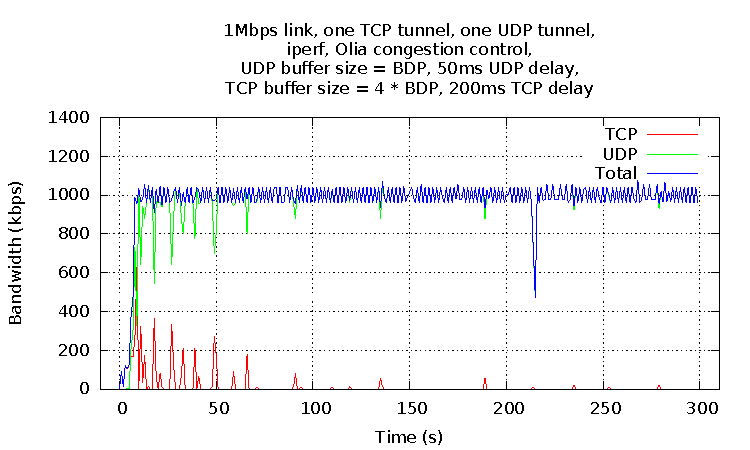
\includegraphics[scale=0.75]{img/olia-mptcp-unequal}
  \end{figure}
\end{frame}

\section{wVegas Behavior}
\begin{frame}{wVegas Behavior - Single TCP Tunnel}
  \begin{figure}
    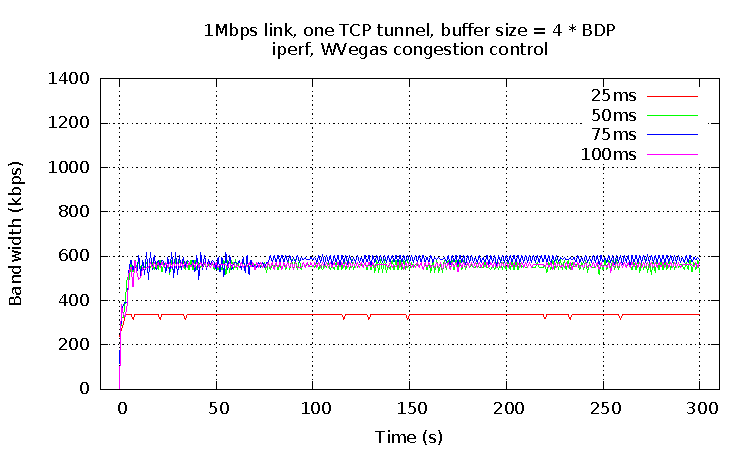
\includegraphics[scale=0.75]{img/wvegas-tcp-4}
  \end{figure}
\end{frame}
\begin{frame}{wVegas Behavior - Two Tunnels}
  \begin{figure}
    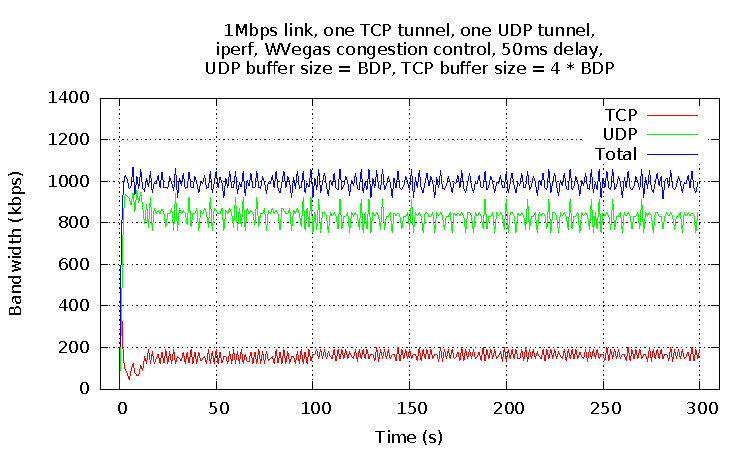
\includegraphics[scale=0.75]{img/wvegas-mptcp-50ms-4}
  \end{figure}
\end{frame}
\begin{frame}{wVegas Behavior - WiFi/3G}
  \begin{figure}
    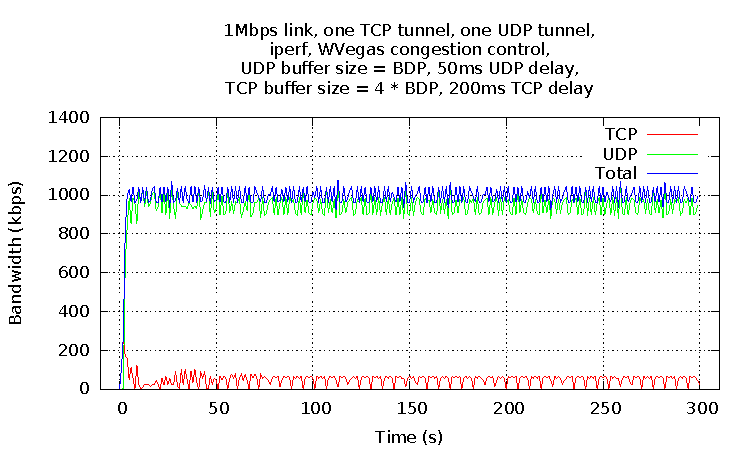
\includegraphics[scale=0.75]{img/wvegas-mptcp-unequal}
  \end{figure}
\end{frame}

\section{Conclusions}
\begin{frame}
  \begin{itemize}
    \item OLIA has improved throughput
    \item wVegas has stable throughput
  \end{itemize}
\end{frame}

\end{document}
